\chapter{MQTT}
Things must be connected to the Internet to become
\textit{``IoT"} devices, and thus to adopt the internet
protocol suite (TCP/IP + application, usually HTTP).
However, the Internet stack is thought for \textit{resource-rich} devices, not for IoT ones.\\
These led the canonical protocol stack to be modified for IoT environments, according to its needs and limitations.

\textbf{MQTT} is a publish-subscribe application protocol, which initially was not designed specifically for IoT.
``MQTT'' stands for \textit{``Message Queuing
Telemetry Transport''}, but ``Queing'' should not be intended literally as it usually is in the ICT world.
{MQTT is built upon TCP/IP. TCP isn't the optimal choice for IoT, UDP is generally preferred, but as said before, MQTT was not designed for IoT:
\ns
\begin{itemize}
   \item Port 1883
   \item Port 8883 for using MQTT over SSL
   \begin{itemize}
      \item \ul{\textit{SSL adds significant overhead!}}
   \end{itemize}
\end{itemize}
}

\labelitemize{\textit{Lightweight}}{
   \begin{itemize}
      \item Small code footprint
      \item Low network bandwidth
      \item Low packet overhead (guarantees better
      performances than HTTP)
   \end{itemize}
} 

\section{Publish-Subscribe recalls}
Publish/subscribe is a \textit{loosely coupled}\footnote{i.e. peers don't have to share ``too much''} interaction schema, where both publishers and subscribers act as ``clients''.
There is a third party called \textit{event service} (aka \textbf{Broker}), which acts as the actual ``server'' (considering the client-server architecture), and which is known by both publishers and subscribers.\\
In this paradigm clients are simple, while the complexity resides in the broker.

\textbf{Publishers}, e.g. a sensor, produce events ---or any data they wish to share by means of events---
and interact only with the broker, while \textbf{subscribers} express the interest for an event, and receive an asynchronous notification whenever an event or a pattern of events is generated;
also subscribers interact only with the broker.\\
\ul{Publishers and subscribers are \textbf{fully decoupled} in \textit{time}, \textit{space} and \textit{synchronization}.}
\begin{itemize}
   \item Space decoupling:
   \begin{itemize}
      \item Publisher and subscriber do not need to know each other
      and do not share anything
      \item they don’t know the IP address and port of each other
      \item they don’t know how many peers they have
   \end{itemize}
   \item Time decoupling:
   \begin{itemize}
      \item Publisher and subscriber do not need to run at the same
      time.
   \end{itemize}
   \item Synchronization decoupling:
   \begin{itemize}
      \item Operations on both pub. and sub. are not halted during
      publish or receiving.
   \end{itemize}
\end{itemize}

The \textbf{Broker}:
\begin{itemize}
   \item \textit{Known} to publishers and subscribers
   \item \textit{Receives} all incoming messages from the publishers
   \item Filters all incoming messages
   \item \textit{Distributes} all messages to the subscribers
   \item Manages the requests of \textit{subscription/unsubscription}
\end{itemize}

\begin{figure}[htbp]
   \centering
   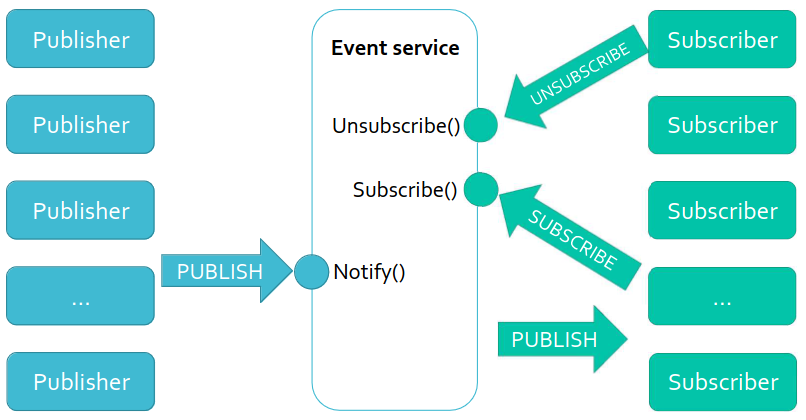
\includegraphics{images/ps_broker.png}
   \caption{Broker management of events}
   \label{fig:ps_broker}
\end{figure}
   
\nl

\subsection{Properties}
Due its decoupling \textbf{properties}, compared to basic \textit{client-server}, publish-subscribe is considered to be more \textbf{scalable}, even if it is implemented using an underlying client-server architecture.

First of all, everything is entirely up to the broker, does not depend on the direct interaction between endpoints.
In case of a very large number of devices, the architecture can scale by \textbf{parallelizing} the (event-driven) operations on the broker.

\nl

Regarding the message filtering performed by the broker, it can happen depending on various fields:
\begin{itemize}
   \item \textbf{Subject topic}
   \begin{itemize}
      \item The subject (or topic) is a part of the messages
      \item The clients subscribe for a specific topic
      \item Typically topics are just strings (possibly organized in a taxonomy)
   \end{itemize}
   \item \textbf{Content}
   \begin{itemize}
      \item  The clients subscribe for a specific query (e.g. $Temp > 30^{\circ}$)
      \item The broker filters messages based on a specific query
      \item Data cannot be encrypted!
   \end{itemize}
   \item \textbf{Data type}
   \begin{itemize}
      \item Filtering of events based on both content and structure
      \item The type refers to the type/class of the data
      \item Tight integration of the middleware and the language (!) 
   \end{itemize}
   \item[] The second and third approaches require \ul{increasing \textbf{integration} mechanisms to provide the desired features}.
\end{itemize}

\section{MQTT and Publish-Subscribe}
MQTT provides a specific implementation of the PS paradigm.
Since it relies on TCP/IP, Publishers and subscribers need to \ul{know the
\textbf{hostname/ip} and port of the broker
\textit{beforehand}}.

Thanks to its speed and to being lightweight, in most applications the delivery of messages is
mostly in \textit{near-real-time}, but in general this is \ul{\textit{not} a guaranteed property}.

In MQTT \ul{message \textbf{filtering} is based only \textbf{topics}}, which is the most flexible filtering of the ones presented in the previous section.

\section{Messages}
A client connects to a broker by sending a \texttt{CONNECT}
message. Since such message may be lost, the broker answers with a \texttt{CONNECTACK} message, indicating simply whether the connection was accepted, refused, and if there was a previously stored session with the client.
{
   \ns
   \begin{itemize}
      \item Client ID
      \begin{itemize}
         \item A string that uniquely identifies the client at the broker.\\
         If empty: the broker assigns a unique \texttt{clientID} and does not keep a status for the client.
         \note{In this case \textit{Clean Session} must be TRUE.
         
         Note also that in \ul{version 3.1.1} the servers replies with a \ul{CONNECTACK with \textit{no} payload}, so the assigned ID is not known to the client.\\
         This has changed in version 5.0}
      \end{itemize}
      \nl

      \begin{center}
         \fbox{

            \begin{minipage}{0.7\columnwidth}
               \subsubsection*{ClientID Uniqueness - Digression}
               \begin{center}
                  \ul{How can a client know if its Client ID is \textbf{unique}?}\\
               \end{center}
               \nl
               The answers is not completely addressed by the standard, and the scenario of a new client who wants to connect and have a persistent session is not clearly discussed.\\
               ClientIDs may be assigned beforehand, but this is possible only if the admin controls \textit{entirely} the system, it is not possible if the broker is \textit{public}, thus an owner of MQTT clients doesn't know whether there are other clients.
               
               In reality, you can ``take your chance'', because the ClientID is 23 byte long, so the chance of an overlap between multiple devices is low.
               
               \vspace*{1.5em}
               
               In general, standard specifications tend to omit everything that can be omitted, to avoid posing constraints which are not strictly necessary, by leaving room for personal implementations and needs.
            \end{minipage}
            }
   \end{center}
\end{itemize}

\nl
\nl
   \labelitemize{\textit{optional}}{
      \begin{itemize}
         \item Clean Session
         \begin{itemize}
            \item Set to \texttt{FALSE} if the client requests a \textbf{persistent session}, allowing for session resuming and better QoS (storing \ul{missed messages with QoS 1,2 not 0!}).
         \end{itemize}
         \item Username/Password
         \begin{itemize}
            \item No encryption, unless security is used at transport layer
         \end{itemize}
         \item Will\footnotemark[1] flags
         \begin{itemize}
            \item If and when the client disconnects ungracefully, the broker will notify the other clients of the disconnection
         \end{itemize}
         \item KeepAlive
         \begin{itemize}
            \item The client commits itself to send a control packet (e.g. a
            ping message) to the broker within a keep-alive interval expressed in seconds,
            allowing the broker to detect whether the client is still
            active (\textbf{detect disconnections})
         \end{itemize}
      \end{itemize}
      }
}
\footnote[1]{This refers to the \textit{Last Will} (Testament), the document with the ``wills'' of someone dead.}

After \texttt{CONNECT} the publishers may send \texttt{PUBLISH} messages, which are later forwarded by the broker to the subscribers, and which are structured as follows:
\labelitemize{\texttt{PUBLISH}}{
   
   \begin{itemize}
      \item \texttt{packetId}
      \begin{itemize}
         \item An integer
         \item It is 0 if the QoS level is 0
      \end{itemize}
      \item \texttt{topicName}
      \begin{itemize}
         \item a string possibly structured in a
         hierarchy with ``/'' as delimiters
         \item Example:
         ``home/bedroom/temperature''
      \end{itemize}
      \item \texttt{qos} 0,1 or 2   
      \item \texttt{payload}
      \begin{itemize}
         \item The actual message in any form
      \end{itemize}
      \item \texttt{retainFlag}
      \begin{itemize}
         \item tells if the message is to be
         stored by the broker as the
         last known value for the topic
         \item If a subscriber connects later,
         it will get this message
      \end{itemize}
      \item \texttt{dupFlag}
      \begin{itemize}
         \item Indicates that the message is
         a duplicate of a previous, unacked message
         \item Meaningful only if the QoS         level is $>0$
      \end{itemize}
   \end{itemize}  
}

\labelitemize{\texttt{SUBSCRIBE}}{
   \begin{itemize}
      \item \texttt{packetId} an integer
      \item \texttt{topic\_1} a string (see publish messages)
      \item \texttt{qos\_1}  0,1 or 2
   \end{itemize}
}

\labelitemize{\texttt{SUBACK}}{
   \begin{itemize}
      \item \texttt{packetId} the same of the SUBSCRIBE message
      \item \texttt{returnCode} one for each topic subscribed
   \end{itemize}
}

There are also \texttt{UNSUBSCRIBE} and \texttt{UNSUBACK} messages which have a similar structure but are not described here.

\section{Topics}
Topics are strings that are organized into a hierarchy
of \textit{``topic levels''}, separated by a \textit{``\texttt{/}''} character.
{\ns\note{Example: \texttt{home/firstfloor/bedroom/presence}}}
Wildcard may be used in the topic levels:
\begin{itemize}
   \item \texttt{home/firstfloor/\textred{+}/presence}\\
   Selects all presence sensors in all rooms of the first
   floor
   \item \texttt{home/firstfloor/\textred{\#}}\\
   Selects all sensors in the first floor
   \item Topics that begins with a ``\texttt{\textred{\$}}'' are reserved for internal statistics of MQTT;
   There is no standardization on such topics, and cannot be published by clients
\end{itemize}

\section{QoS}
The \textbf{QoS} is an agreement between the sender and the
receiver of a message.
\note{For example, in TCP the QoS includes guaranteed delivery and ordering of messages.}

In MQTT the QoS is an agreement \ul{between the clients and the broker}, and there are three levels:
\begin{enumerate}[label={\texttt{level \arabic*}},start=0]
   \item \textbf{At most once}
   \begin{itemize}
      \item It is a ``best effort'' delivery and messages are \textit{not} acknowledged by the receiver
   \end{itemize}
   \item \textbf{At least once}
   \begin{itemize}
      \item Messages are numbered and stored by the broker until
      they are delivered to all subscribers with QoS level 1. Each message is delivered at least once to the subscribers with QoS, but possibly also more. 
   \end{itemize}
   \item \textbf{Exactly once}
   \begin{itemize}
      \item  guarantees that each message is received \textit{exactly once} by the recipient, exploiting a double two-way handshake.
   \end{itemize}
\end{enumerate}

{Note that QoS is used both:
\ns
\begin{itemize}
   \item between publisher and broker
   \item between broker and subscriber
\end{itemize}
But the \ul{\textbf{QoS} in the two communication \textbf{may be different}}.
}
\begin{figure}[htbp]
   \centering
   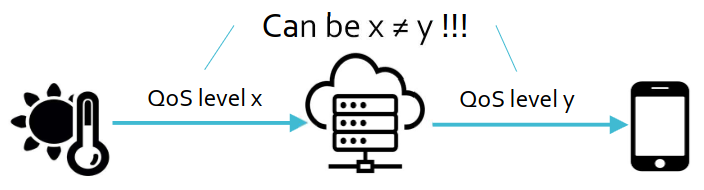
\includegraphics{images/qos_different.png}
   % \caption{}
   \label{fig:qos_different}
\end{figure}

\subsection{Choosing the right QoS}
\begin{itemize}
   \item Use QoS level 0 when:
   \begin{itemize}
      \item The connection is stable and reliable
      \item Single message is not that important or get stale with
      time
      \item Messages are updated frequently and old messages
      become stale
      \item Don’t need any queuing for offline receivers
   \end{itemize}
      \item Use QoS level 1 when:
   \begin{itemize}
      \item You need all messages and subscribers can handle
      duplicates
   \end{itemize}
   \item Use QoS level 2 when:
   \begin{itemize}
      \item You need all messages and subscribers cannot handle
      duplicates
      \item Has much higher overhead!!!!
   \end{itemize}
\end{itemize}

\section{Persistent Sessions}
Persistent sessions keep the state between a client and the broker:
if a subscriber disconnects, when it connects again, it does not need to subscribe again the topics.\\
The session is associated to the clientId defined with the \texttt{CONNECT} message, and stores:
\begin{itemize}
   \item All \textbf{subscriptions}
   \item All QoS 1\&2 messages that are \textbf{not confirmed} yet
   \item All QoS 1\&2 messages that arrived when the \textbf{client was
   offline}
\end{itemize}

Note that \ul{with \texttt{QoS = 0} persistent sessions are useless overhead}.

\section{Retained messages}
A publisher has \textbf{no guarantee} wether its messages are ---or \textit{when}---
actually delivered to the subscribers,
it can only achieve guarantee on the delivery to the broker.

A \textbf{retained message} is a normal message with
\texttt{retainFlag = True}; the message is stored by the broker, and if a new retained message of the same topic is published, the broker will keep only the last one.
When a a client subscribes the topic of the retained
message  the broker immediately sends the retained message,
allowing subscribers to immediately get updated to the ``state of the art''.

Note that \ul{retained messages are kept by the server even if they had already been delivered.}

\section{Last will \& testament}
Last Will \& testament is used to notify other clients about the \textbf{ungraceful disconnection} of a client.

The broker stores the \textbf{last will message} attached to the \texttt{CONNECT} message, but if the client gracefully closes the connection by sending \texttt{DISCONNECT}, then the stored \textit{last will message} gets discarded.

Often the \ul{Last Will message is used along with retained messages}.

\section{Packet Format}
\begin{figure}[htbp]
   \centering
   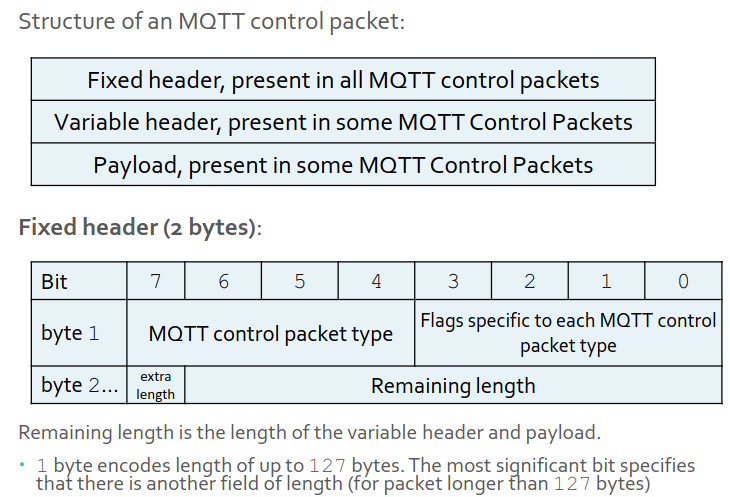
\includegraphics[width=0.45\columnwidth]{images/mqtt_packetformat1.png}
   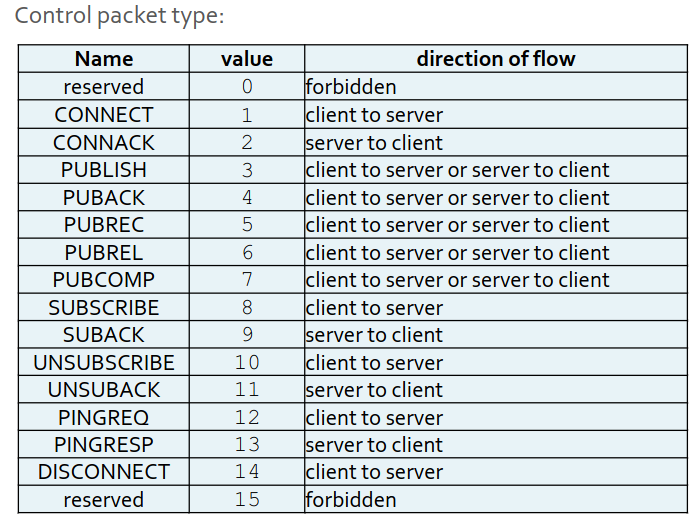
\includegraphics[width=0.45\columnwidth]{images/mqtt_packetformat2.png}\\
   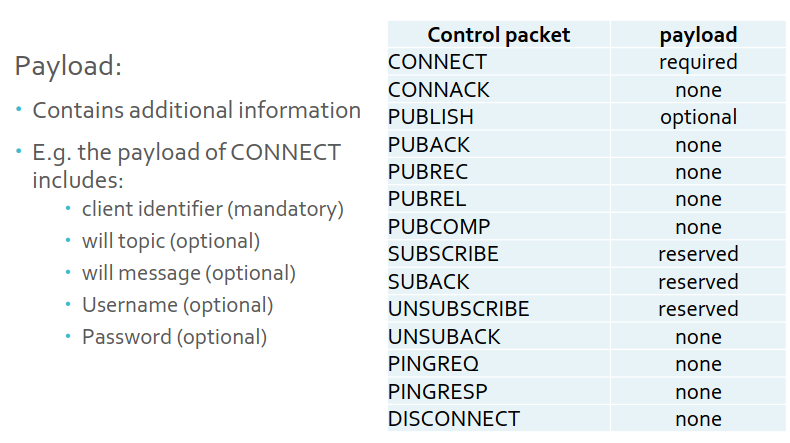
\includegraphics[width=0.45\columnwidth]{images/mqtt_packetformat3.png}
   \caption{MQTT Packet headers}
   \label{fig:mqtt_packetformat}
\end{figure}

The ---not displayed in Fig. \ref{fig:mqtt_packetformat}--- \textbf{Variable header}:
\begin{itemize}
   \item Contains the packet identifier (encoded with two
   bytes)
   \begin{itemize}
      \item Only CONNECT and CONNACK control packets do not
      include this information
      \item The PUBLISH packet contains this information only if $\texttt{QoS}>0$
   \end{itemize}
   \item Contains other information depending on the control
   packet type
   \begin{itemize}
      \item For example, CONNECT packets include the protocol name and version, plus a number of flags (see CONNECT)
   \end{itemize}
\end{itemize}

